The Hybrid Attention Transformer proposed by Chen et al. \cite{chenHATHybridAttention2024},
combines the shifted window mechanism as used in SWinIR by Liang et al. \cite{liangSwinIRImageRestoration2021a}
and Channel Attention \cite{zhangImageSuperResolutionUsing2018},
in a Hybrid Attention Block where both operations are performed in parallel.
On top of that they introduce Overlapping Cross-Attention, which we already discussed in section \ref{sec:transformer}.

\begin{figure}[h!]
    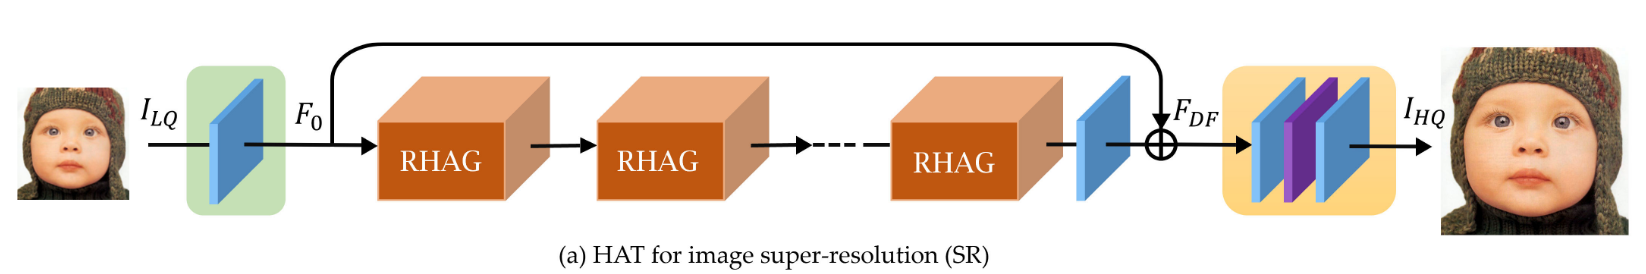
\includegraphics[width=0.9\textwidth]{models/sisr/imgs/hat.png}
    \caption{Image taken from \cite{chenHATHybridAttention2024}, architecture of HAT model.}
    \label{fig:hat_model}
\end{figure}

The overall architecture is shown in figure \ref{fig:hat_model}.
The architecture follows the general scheme described in section \ref{sec:general_model},
initial feature extraction is performed via a single convolutional layer,
spatial upsampling is achieved using subpixel convolution.
The deep feature extraction module proposed by Chen et al. \cite{chenHATHybridAttention2024}
is composed of $6$ cascaded Residual Hybrid Attention Groups (RHAG)

    $$ H_D = H_{RHAG} \circ ... \circ H_{RHAG} ~. $$

A RHAG is made up of $6$ Hybrid Attention Blocks (HABs) followed by one OCA-Block as defined in \ref{def:oca_block} 
and a convolutional layer

    $$ H_{RHAG} = C(180, 180) \circ \text{OCAB}(180, 6, \Phi) \circ H_{HAB} ... \circ H_{HAB}  ~. $$

A HAB is a modification of a Shifted Window Transformer Block, 
where in parallel to the Shifted Window Multi Headed Attention,
Channel Attention Block (CAB) $H_{CAB}$ is employed

    \begin{equation} \label{eq:cab}
        H_{CAB} = H_{CA} \circ C \circ \text{ReLU} \circ C ~,
    \end{equation}

with $H_{CA}$ defined as in equation \ref{eq:ca}.
Let $s: \mathbb R^{d} \times \mathbb R^{d} \to \mathbb R^d, s(x,y) = x + y$ be the element-wise summation

    $$H_{HAB} = R( \Phi \circ \text{LN} ) \circ R( s \circ P(H_{CAB}, \text{SWinMSA}) \circ \text{LN} ) ~. $$

The exact architecture of the network $\Phi$ is not specified by Chen et al. \cite{chenHATHybridAttention2024}.
A construction as in equation \ref{eq:phi} can be used.
The modules $H_{RHAG}, H_{HAB}, \text{OCAB}$ and $H_{CAB}$ are visualized in figure \ref{fig:hat_modules}.

\begin{figure}[h!]
    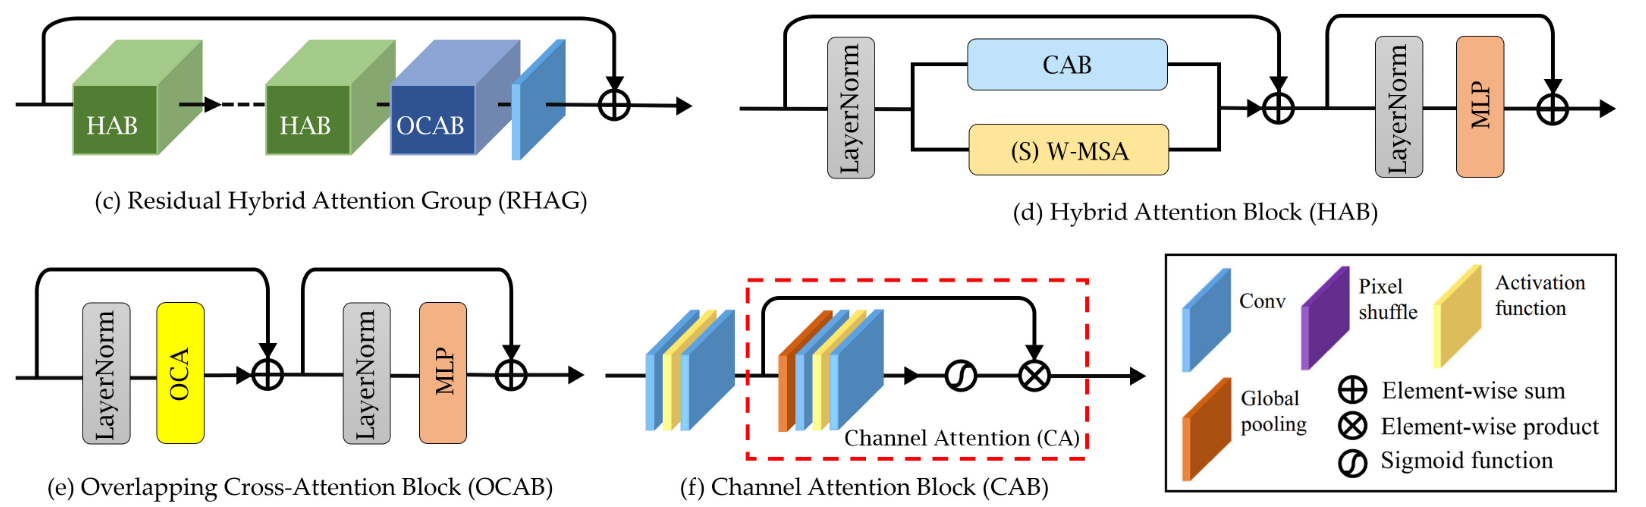
\includegraphics[width=0.9\textwidth]{models/sisr/imgs/rhag.png}
    \caption{Image taken from \cite{chenHATHybridAttention2024}, Residual Hybrid Attention Group.}
    \label{fig:hat_modules}
\end{figure}